\chapter{Prototypen} 

I dette kapittelet vil det bli gitt en innføring i valg som ble tatt før og underveis i utviklingen av prototypen. 
 
\section{Utgangspunkt} 
\label{sec:utgangspunkt} 

Målet med oppgaven var å undersøke potensielle forbedringer som kunne implementeres i programvaren Sono Flex. Det mest naturlige valget ville da  ha vært å utviklet de ønskede endringene i den eksisterende koden. Tobii Dynavox ville derimot at de skulle implementeres på en annen plattform. Den ene grunnen var at den eksisterende teknologien hadde flere begrensninger som ville gjort det vanskelig å fått implementert mye av funksjonalitet som skulle undersøkes. Spesielt gjelder dette animasjonene. Den andre var at Windows Forms, som Sono Flex er bygget på,  er satt til å  kun vedlikeholdes av Microsoft  \cite{AAAWPF8:online}.  Det vil si at bugs og feil blir fikset, men at ingen nye funksjoner vil bli lagt til. Dette kan også tyde på at den utfases og at de har valgt å fokusere utviklingen på en annen teknologi. Tobii var derfor interessert i å finne en annen plattform å bygge programvaren på.

Utviklingen startet derfor som et nytt prosjekt og at første del ble å lage en high-fidelity prototype ved å bruke "reverse engineering" på Sono Flex. Det vil si at funksjonaliteten og det meste av utseende skulle være det samme, men at implementasjonen og teknologien ville bli annerledes.


\section{Kravspesifikasjon} 


Å utvikle all funksjonaliteten som Sono Flex tilbyr ville vært for ressurskrevende og derfor utfor denne oppgavens omfang. Det ble derfor bestemt å kun fokusere på det mest nødvendige og heller opprettholde god kodekvalitet. For å finne ut hva som var mest nødvendig og av interesse ble det i samtaler med Tobii funnet en del krav og funksjoner som de ønsket. Disse er spesifisert i listen under og er sortert etter prioritering. 
 
\subsection{Funksjonelle krav} 
 
\textbf{Bygge setninger} – En bruker skal ha mulighet til å sette sammen enkle setninger. Helst skal kompleksiteten til  en setningen begrenses av brukerens vokabular og ikke av systemets mangler.
 
\textbf{Øyesporing som interaksjon} - Det skal være mulig å operere prototypen ved å \underline{kun} bruke øynene. En som tar i bruk øyesporing skal ha tilgang  på samme funksjonaliteten som hvis han hadde tatt i bruk datamus. Det skal også jobbes for å få effektiviteten så lik som mulig mellom de to interaksjonsformene. 
 
\textbf{Bilde for vært ord} - For vært ord skal det være en billedlig fremstilling av det. En bruker, skal i teorien, kun ved å se på bildet forstå hvilket ord det representerer. 

\textbf{Norsk} – Det skal være støtte for norsk. Ord og all tekst skal være på norsk.
Det bør også legges opp til at en enkelt kan skifte språk. 

\textbf{Tale} - Systemet skal kunne gjøre setninger som brukeren har skrevet om til lyd. Jo mer naturlig talen høres ut jo bedre.
  
\textbf{Brukertilpasning} - Hver bruker skal ha mulighet til å kunne tilpasse programvaren etter sine preferanser.
  
\textbf{Animasjon og Lydeffekter } - I prototypen skal en bruker ha mulighet til å aktivere animasjoner og lydeffekter. Disse skal bli avspilt når en bruker trykker på de ulike symbolene.  Neste kapittel vil spesifisere dette i detalj.

\textbf{Logging} - I systemet skal det være mulig å kunne logge all interaksjonen en bruker gjør med programvaren. Denne funksjonen vil være nødvendig for å kunne gjennomføre testingen 

\subsection{Ikke-funksjonelle krav} 
 
\textbf{Kodekvalitet} - Kodebasen skal være tilrettelagt for vedlikehold og videreutvikling. En viktig del av oppgaven var at personer som ikke har deltatt i systemutvikling skal ha mulighet til å forstå koden slik at de enkelt kan legge til og fikse funksjoner. Programvaren skal også legge opp til at det er enkelt og bytte ut animasjoner, lyd og nye symboler. 

\textbf{Brukervennlighet} - Målgruppen består av barn som har begrenset erfaring med å operere dataprogrammer. Det er derfor viktig at det legges vekt på dette og at programvaren utformes på en måte som er intuitiv for brukeren.   
 
 \textbf{Responstid} -  Programvaren er kompleks og det tar lang tid å skrive med symboler, det er derfor viktig at systemet responderer kjapt og ikke gjør at oppgaven tar lenger tid enn nødvendig. Når brukeren trykker på noe skal det føles som om programvaren svarer momentant. 

\textbf{Personvern} - Brukerne av programvaren er en sårbar gruppe, det vil derfor være viktig at sensitiv informasjon ikke kommer på avveie. Det skal i utgangspunktet ikke lagres sensitiv data, men hvis data lagres skal det lagres på en sikker måte. 
 
\section{Utvikling} 
I denne seksjonen vil teknologier og arbeidsområde bli beskrevet.  
 
\section{Programmeringsrammeverk} 

Et programmeringsrammeverk var ikke nødvendig for å kunne bygge prototypen, men har flere fordeler som gjorde at det ikke kunne utelates. Blant det viktigste er lav-nivå kode som allerede har blitt testet og brukt av andre programmerere \cite{Frame7:online}. Dette øker påliteligheten til koden og reduserer utviklingstiden.
Til å utvikle prototypen ble programmeringsrammeverket .NET brukt. Dette ble valgt på grunn av at dokumentasjonen til øyesporingsenheten anbefaler det og alle eksemplene i dokumentasjonen bruker det. En annen grunn var at dette rammeverket tilbyr flere gode brukergrensesnitt-teknologier som var ønskelig med tanke på at prototypen som skulle utvikles var svært grafisk.

\subsection{.NET}
 
Som en kan se på figur \ref{fig:net-arkitektur}  er arkitekturen til .NET omfattende og har flere programmeringsspråk og komponenter en kan velge å ta i bruk. Rapporten vil kun gi informasjon om de ulike komponentene fra .NET som ble brukt eller som er nødvendig for forståelse av valgene som har blitt tatt. 
 
 
\begin{figure}[ht] 
\centering 
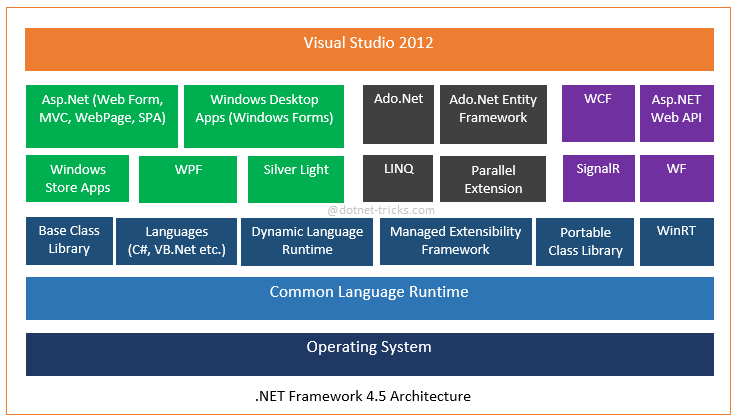
\includegraphics[width=140mm]{netframework45} 
\caption{Diagram som viser arkitekturen til .net rammeverket versjon 4.5} 
\label{fig:net-arkitektur} 
\end{figure} 
 
 
\section{Brukergrensesnitt-teknologi} 

Brukergrensesnitt-teknologi gir utvikleren tilgang på funksjoner og forhåndsdefinerte grafiske elementer som skal gjør utviklingen mer effektiv. Som en kan se ut ifra figur \ref{fig:net-arkitektur} tilbyr .NET teknologier som Windows Store Apps, Windows Presentation Foundation(\gls{WPF}), Windows Forms og Silverlight. Alle disse ble evaluert før et endelig valg ble foretatt:

\textbf{Windows Forms} ble utelukket ettersom dette er teknologien som Sono Flex er bygget på og som hadde begrensinger som gjorde at flere av de ønskede funksjonene ble vanskelig å implementere. 

\textbf{Windows Store Apps} hadde mye av den ønskede funksjonaliteten, samtidig som den fortsatt vedlikeholdes. Problemet var at for å distribuere slike applikasjoner brukes Windows Store og for å få publisert applikasjonen der, kreves godkjenning av Windows. Dette i sammenheng med at disse applikasjonene ikke er kompatible med Windows 7\cite{Windo0:online} gjorde at denne teknologien ikke ble valgt. 

\textbf{Silverlight} er ifølge Microsoft sin blogg\cite{User1111:online} en kraftig utviklingsplattform for å lage "rike" media- og forretningsapplikasjoner for web, skrivebord og mobil. Fokuset til teknologien er derimot på web og mobil \cite{Micro6:online}, og ettersom prototypen er en skrivebords applikasjon falt ikke valget på Silverlight.

Teknologien som til slutt ble valgt var \textbf{Windows Presentation Foundation}. WPF skal tilby utviklere en helhetlig programmeringsmodell for å bygge skrivebords applikasjoner for Windows som tar i brukergrensesnitt, media og dokumenter \cite{Windo777:online}. Grunnen til at teknologien ble valgt er:


\begin{itemize}
\item Fokus på skrivebord. I motsetning til blant annet Silverlight, er WPF designet og laget for å utvikle klient applikasjoner\cite{Windo777:online}.
\item Prioritert av Tobii PC Eye GO. I dokumentasjonen til øyesporingsenheten er det skrevet: "WPF  rammeverket er et svært bra verktøy for utvikling av grafikk-intensive applikasjoner og WPF har derfor blitt gitt høyest prioritet [..]"
\item Etterfølgeren til Windows Forms . WPF er ifølge Microsoft erstatteren til teknologien som blir brukt i Sono Flex \cite{User1111:online}. 
\item God støtte for animasjoner. WPF tilbyr blant annet et eget timing system for å enkelt holde tiden når en animerer grafiske elementer \cite{Anima7:online}.
\end{itemize}



 
\subsection{Windows Presentation Foundation} 
 
Ifølge Adam Nathan \cite[p.~9]{WPFbook}, programvare arkitekt hos Microsoft, ble prosessen med å lage WPF igangsatt fordi ingen hadde adressert vanskeligheten med å lage moderne brukergrensesnitt. Spesielt med tanke på at grafisk maskinvare hele tiden har blitt bedre og billigere sammen med at forbrukernes forventninger har fortsatt å stige. 
Han argumenterer med at det fantes utviklere på tiden som for eksempel brukte bitmap bilder for å endre utseende på standardknappene. Problemet er at disse formene for tilpasning ikke bare kan være ressurskrevende å utvikle, men også gi en dårligere brukeropplevelse. Han forteller videre at de ønsket å lage et rammeverk som hadde produktiviteten som folk likte med Windows Forms og som var like enkel som HTML og Javascript.

WPF gir utvikleren mulighet til å utvikle applikasjoner med både markup- og programmeringspråk. Markup språket brukes vanligvis til å implementere utseende til applikasjonen, mens programmeringsspråket brukes vanligvis til å implementere oppførselen. Det vil si at det er mulig å bruke de på tvers, men WPF legger opp til å skille mellom utseende og oppførsel \cite{Intro8:online}. Dette skillet skal ifølge utviklerne gi flere fordeler som blant annet reduksjon av utvikling- og vedlikeholdskostnader. Fordi utseende-spesifikk markup ikke er tett koblet med oppførsel-spesifikk kode. Skillet mellom dem gir også designere mulighet til å jobbe med utseende samtidig som utviklere jobber med oppførsel \cite{Intro8:online}. I WPF er eXtensible Application Markup Language (XAML) brukt som markup språk. Mens man som programmeringsspråk kan velge mellom C-Sharp eller Visual Basic.

\subsubsection{C-Sharp} 

Valget av programmeringsspråk sto mellom C-Sharp og Visual Basic (VB), to språk med svært forskjellig syntaks og historie \cite{Compa6:online}. C-Sharp har basert syntaksen sin på programmeringsspråket C , mens VB har sine røtter fra programmeringsspråket BASIC \cite{Visua3:online} \cite{About8:online}. Begge språkene har de samme mulighetene, forskjellen ligger hovedsakelig i syntaks, så valget av programmeringsspråk ble basert på preferanser \cite{What0:online}. I dette tilfelle ble det valgt å ta i bruk C-Sharp, mest på grunn av likheten med Java som vi hadde erfaring med fra tidligere.


\subsubsection{eXtensible Application Markup Language (XAML)} 

XAML, en dialekt av XML, har vært en viktig del av WPF siden dens introduksjonen i 2006 \cite[p.~17]{WPFbook}. Vanligvis brukes XAML til å spesifisere brukergrensesnitt objekter og organiseringen av dem, men kan også brukes til andre ting som for eksempel animasjoner \cite{Story5:online}. 

Grunnen til at XAML har blitt brukt er fordi det er enkelt for programmere å samarbeide med eksperter fra andre felt. Nathan forteller at XAML blir fellesspråket for alle partiene, hovedsakelig gjennom utviklingsverktøy og felt-spesifikke design verktøy. Men også fordi XAML (og XML generelt) er enkelt å lese og forstå \cite[p.~17]{WPFbook}. Figur \ref{listing:knapp} viser hvor enkelt en kan genere en blå knapp som også er lettleselig .


\begin{listing}[ht] 
\inputminted[fontsize=\footnotesize, frame=lines,framesep=2mm,baselinestretch=1.2,bgcolor=lightgray,linenos]{xml}{Code/xamlexample.xml} 
\caption{Hvordan en blå knapp blir definert i XAML} 
\label{listing:knapp} 
\end{listing} 
 
   
\section{IDE og versjonskontroll} 

For å automatisere mye av utviklingen ble det valgt å bruke utviklingsmiljøet Visual Studio 2013 \cite{2013-1:online}. Grunnen til at Visual Studio ble valgt er det fordi den i tillegg til å ha et kode-redigeringsverktøy og debugger, så har den også en WPF designer\cite{What8:online}. Denne designeren tilbyr flere hjelpemidler for å effektivisere prosessen med å lage brukergrensesnitt. Blant annet kan man velge mellom å manuelt skrive grafiske elementer i XAML eller man kan trekke inn forhåndsdefinerte elementer fra et sidepanel. Den viktigste funksjonen som tilbys er derimot design vinduet. Dette viser til enhver tid hvordan brukergrensesnitt blir uten å måtte kjøre koden\cite{WPF D1:online}. 
 
For versjonskontroll ble det av erfaringsmessige årsaker brukt git\cite{AboutGit:online}. Til å ta backup av prosjektet ble den web-baserte tjenesten Bitbucket brukt. Grunnen til dette var at mye av koden fra Tobii Dynavox var konfidensiell og Bitbucket tilbyr hemmelig oppbevaring gratis. 
 
 
\section{Model View ViewModel} 

En viktig del av oppgaven var å utvikle en prototype som Tobii Dynavox kunne bygge og teste videre på. Det var derfor en forutsetning at kildekoden var tilrettelagt for vedlikehold og videreutvikling. Et tiltak som ble gjort for å gjennomføre dette var å følge arkitekt mønsteret Model view Viewmodel (MVVM). Grunnen til at vi valgte dette fremfor mønster som for eksempel Model View Contoller(MVC)\{MVC a2:online} og Model-View-Presenter(MVP)/cite{The M4:online}. Er fordi MVVM ble utviklet av Microsoft spesifikk for å utnytte funksjonaliteten til WPF  og at mønsteret er som skreddersydd for teknologien \cite{THEM6:online}. 

Det ble tidligere nevnt a WPF legger opp til å skille mellom utseende og oppførsel, MVVM skal hjelpe utviklere å følge dette prinsippet. Ved å skille mellom applikasjons logikk og brukergrensesnitt skal det ifølge Microsoft \cite{Im1online}, være enklere å teste, vedlikeholde og videreutvikle. MVVM gjør dette ved å dele opp koden i 3 deler - Modeller, ViewModel og View. Figur \ref{fig:mvvm} viser de tre MVVM klassene view, view-model og model, og interaksjonen mellom disse.
 
\begin{figure}[ht!] 
\centering 
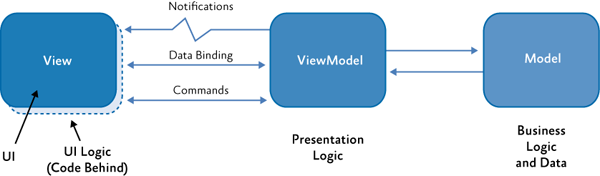
\includegraphics[width=100mm]{Mvvm} 
\caption{Illustrasjon som viser tre MVVM klasser og hvordan interaksjonen mellom dem\cite{Im1online}} 
\label{fig:mvvm} 
\end{figure}


\subsection{Model}

\textit{Model} delen av MVVM står for en av de viktigste delene i enhver applikasjon, nemlig data og informasjon. \textit{Model} sin eneste jobb er å representere og holde dataene som applikasjonen skal bruke. Den skal ikke hente data fra en database eller manipulere data på noen som helst måte \cite{Model7:online}. Dette går under forretningslogikk og skal ifølge mønsteret holdes separat fra model-klasser. 


\subsection{View}
 
 Som navnet impliserer, skal klasser definert som \textit{View} stå for visuelle elementer som vinduer, knapper, tekst, farger og organiseringen av dem. Med andre ord, selve brukergrensesnittet \cite{THEM6:online}. View-klasser vil bli skrevet i XAML.

 
\subsection{ViewModel}
 
 Som en kan se utfra figur \ref{fig:mvvm} ligger \textit{Viewmodel} mellom \textit{Model} og \textit{View}. Så mens \textit{model} holder data og \textit{View} presenterer data så er det \textit{Viewmodel} sin jobb å manipulere og håndtere data. Si for eksempel at \textit{Model} holder en dato lagret i et format som ikke er så lettleselig. Det er da \textit{ViewModel} sin jobb å konvertere det til et mer leselig format før \textit{View} presenterer det til leseren. 
 
\subsection{Databinding, Notifikasjon og Kommando}

Et \textit{View} og en \textit{ViewModel} skal ifølge mønsteret ha en en-til-en relasjon, der \textit{view} har en referanse til \textit{ViewModel}, men ikke omvendt. For at \textit{ViewModel} og et \textit{View} skal kunne "snakke" sammen og fortsatt holdes separat brukes databinding, kommandoer og notifikasjoner. 

\textit{View} presenterer informasjon til brukeren ved å binde seg til egenskaper og kommandoer som \textit{Viewmodel} eksponerer, dette kalles for \textbf{databinding}. Når en egenskap endres i \textit{ViewModel} vil \textit{View} bli oppmerksom på dette gjennom en notifikasjon og oppdateres deretter. 

En kommando er implementert i \textit{ViewModel}, men blir aktivert fra \textit{View}. Dette skjer ved at en bruker trykker på en knapp, \textit{View} klassen vil så forteller \textit{ViewModel} å kjøre en gitt kommando.

\subsection{MVVM-light toolkit} 
 
 MVVM-light er et bibliotek som skal hjelpe utviklere med å sette opp MVVM i kodebasen \cite{Nico0:online}. Hensikt ved biblioteket er å akselerere utviklingen av MVVM applikasjoner i WPF, Silverlight, Windows Store, Windows Phone og Xamarin \cite{MVVM8:online}. Dette skal det gjøre ved å levere et utviklingsklart fundament og flere hjelpeklasser. 


Den viktigste grunnen til at dette tredjeparts biblioteket ble tatt med i prosjektet er på grunn av en funksjon kalt DesignTime-Data \cite{MVVMLightDoc:online}. For en av fordelene ved å skrive brukergrensesnittkode i XAML er at en har mulighet til å se resultatet momentant i et design vindu. Ulempen er at dette kun gjelder for statisk innhold og ikke data som må hentes fra databaser, web-tjenester eller andre kilder. Ved å bruke DesignTime-data kan man bruke en boolsk egenskap som heter IsInDesignModeStatic \cite{MVVM100123:online}. Hvis denne er sann så kan man hente dummy data, hvis ikke så kan det hentes fra den faktiske kilden. Dette gjør at man slipper å kjøre programmet for å se endringer. 


\section{Dataformat og lagring}


Programvaren skal strebe etter å kunne tilby de ordene en bruker har lyst å bruke. En ganske stor utfordring med tanke på at et barns vokabular allerede i alder av 5 år kan være opp i mot 2000 ord. Spesielt med tanke på at hvilket ord dette er, vil variere fra person til person. For vært ord må det også være et symbol som representerer det. En naiv fremgangsmåte ville vært å statisk gjengi hver brikke med et ord og bilde. Problemet med dette er først og fremst at XAML koden blir svært lang, som følge av at en må skrive en knapp for vært tilfelle. Den andre er at en også må inn i koden for å gjøre endringer eller legge til nye ord. 

Løsningen på ble å oppbevare alle ordene i en separat fil for å skille mellom brukergrensesnitt og data. Det ble laget to variasjoner for lagre data - den ene i JavaScript Object Notation(JSON) dokument den andre som et tekstdokument.

\subsection{JSON}

JSON er et lettvekt data-utvekslings format som er lett for mennesker å lese og skrive, og som er lett for maskiner å tolke og generere\cite{JSON7:online}. Figur \ref{listing:jsonfile} viser et utdrag fra en av JSON filene som brukes i prototypen. Hver JSON fil består av en liste med JSON objekter som har attributtene \textit{Name} og \textit{Image}. Der \textit{Name} er ordet og \textit{Image} er stien til et bilde som representerer ordet. Dette er bare et lite utdrag fra filen og viser kun det som ville tilsvart fire brikker i programvaren.

I dette dokumentet er det første objektet "I" et ord, mens de tre neste er kategorier. Hver kategori består av flere ord. Ordene som tilhører en kategori er lagret i en egen fil i en mappe med samme navn. 

Figur \ref{fig:jsonstructure} viser strukturen på filene, der hver kategori har sin egen mappe. Dette gjør at data hentes "just-in-time". Det vil si at istedenfor at ordene ligger i minnet til enhver tid, så hentes de kun når ved behov. Eksempelvis hvis en bruker trykker på kategorien "Food and Drink" så vil ordene hentes fra "FoodAndDrink.json" i mappen "FoodAndDrink". Noe som sparer på minnet, men som kan forringe kjøretiden. For når det er snakk om så store mengder data som alle ordene ville gitt, er det ikke gunstig å bevare dem i minnet. 


\begin{listing}[ht] 
\inputminted[fontsize=\footnotesize, frame=lines,framesep=2mm,baselinestretch=1.2,bgcolor=lightgray,linenos]{json}{Code/JSONfile.json} 
\caption{Utdrag fra filen som inneholder ord og sti til bilde som representerer det i JSON format} 
\label{listing:jsonfile} 
\end{listing} 
 

 \begin{figure}[ht!] 
\centering 
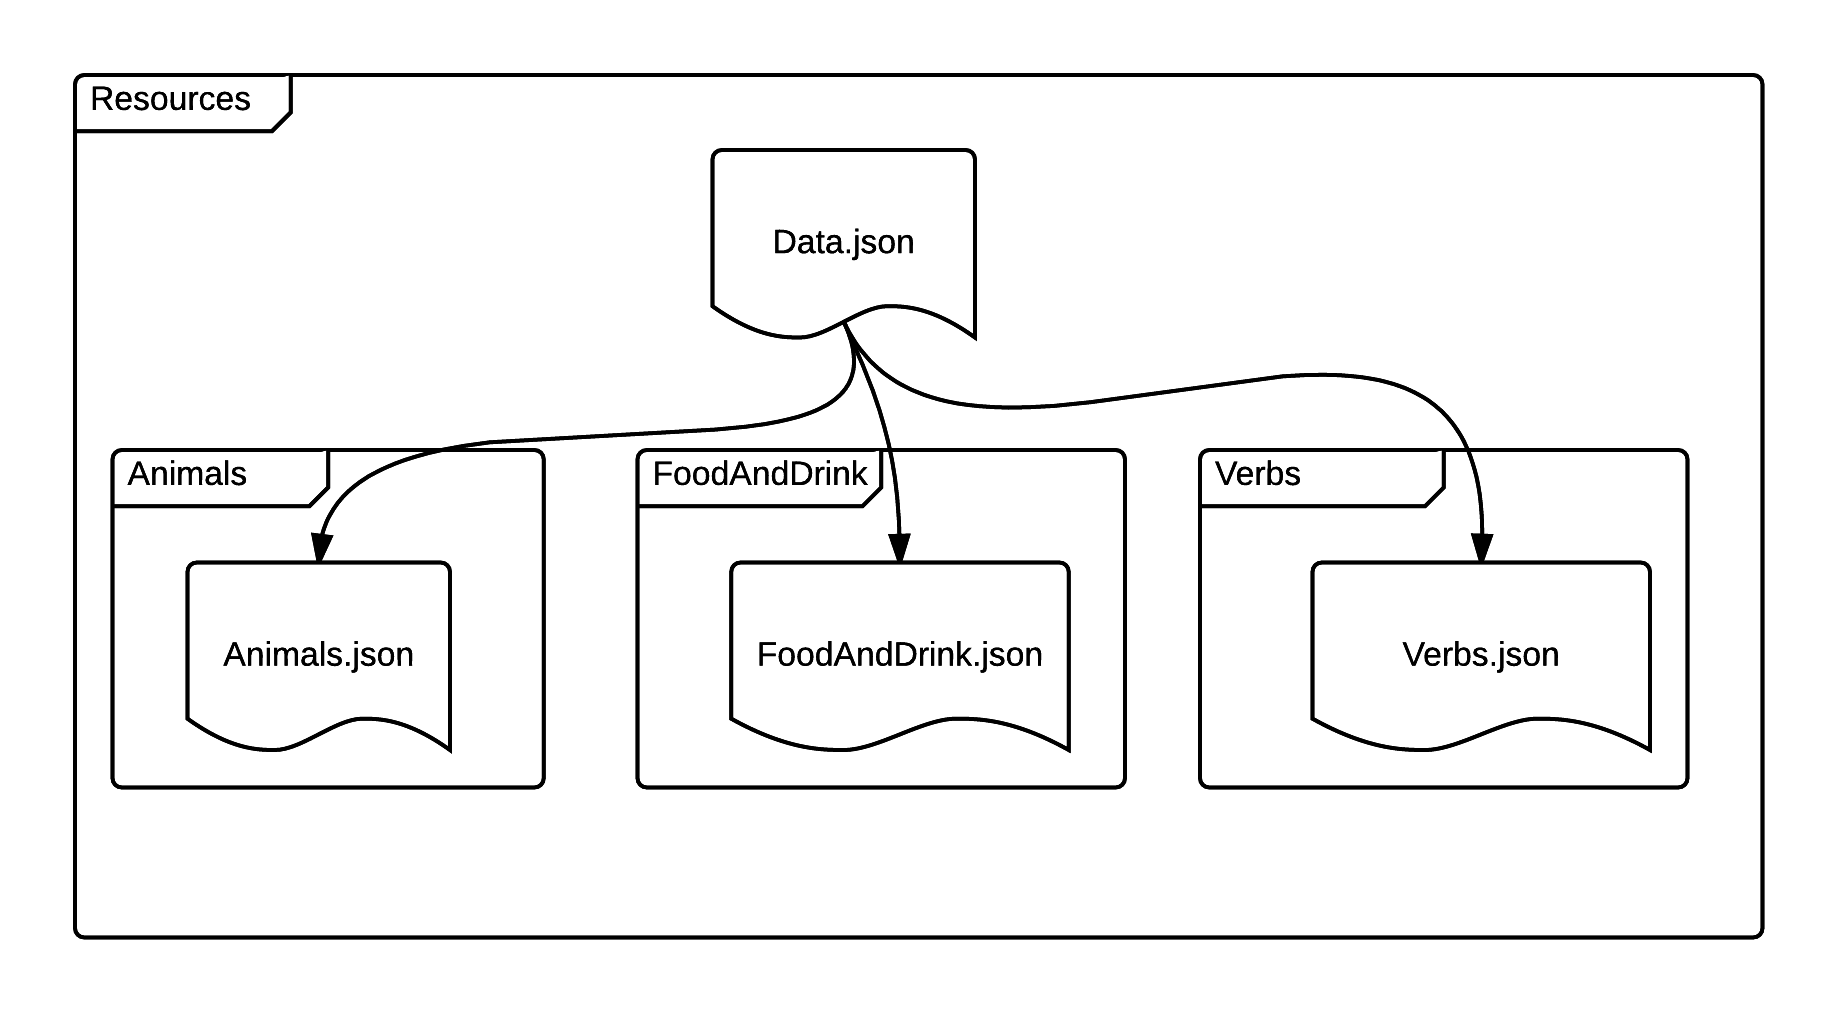
\includegraphics[width=100mm]{JsonStructure} 
\caption{Mappestruktur til et utvalg kategorier} 
\label{fig:jsonstructure} 
\end{figure} 


\subsection{JSON Tolking}

For å kunne ta i bruk objektene definert i tekstfilen må de tolkes om fra JSON format til dataobjekter. Denne prosessen, å trekke ut datastrukturer fra bytes, kalles deserialisering. For å gjøre dette har vi brukt et tredjeparts rammevekt kalt JSON.NET \cite{Json.0:online}. Det finnes en innebygd funksjon i .NET kalt DataContractJsonSerializer \cite{DataC3:online} som også greier å deserialisere et JSON dokument. Grunnen til at JSON.NET ble brukt er fordi i dette biblioteket er det mulighet å automatisk deserialisere en helt liste av JSON objekter til en dataliste uten å manuelt måtte legge inn objektene. Ifølge utviklerens egne nettsider skal rammeverket være 50 prosent kjappere enn DataContractJsonSerializer, men ytelsen er avhengig av hvilke datasett som brukes, og har ikke vært en faktor i avgjørelsen. 


\begin{listing}[ht] 
\inputminted[fontsize=\footnotesize, frame=lines,framesep=2mm,baselinestretch=1.2,bgcolor=lightgray,linenos]{csharp}{Code/JSONparser.cs} 
\caption{Koden som konverterer JSON filen til en Liste} 
\label{listing:JsonParser} 
\end{listing} 


Koden i figur \ref{listing:JsonParser} deserialiserer JSON dokumentet om til en dataliste. Fra linje 5 til 12 skrives teksten fra filen over til en \textit{string}. På linje nummer 14 blir strengen konvertert til et dataobjekt. Dokumentet blir gjort om fra \textit{string} til et komplekst objekt på kun en linje. 


\section{Tekstfil}

Under utviklingen ble det bare lagt inn tilfeldige ord og bilder hentet fra internett i prototypen, men ettersom prototypen begynte å bli ferdigstilt var det behov for et større utvalg ord og symboler. Det ble derfor gitt tillatelse av Tobii Dynavox til å ta i bruk det samme bildene som de bruker i deres programvare. Sammen med bildene fulgte det med et dokument som hadde en beskrivelse av vært bilde og ordet det representerer. For vært ord var egenskapene beskrevet i liste \ref{itm:egenskaper} tilgjengelig. 

\begin{itemize}
\label{itm:egenskaper}
\item Symbol ID
\item Dato oppdatert
\item Dato laget
\item Kategori Navn 
\item Filnavn
\item Filsti
\item Ord
\item Synonymer
\item Tysk, nederlandsk, norsk, svensk, dansk, engelsk, spansk, italiensk, fransk, portugisisk.
\end{itemize}


Hver av egenskapene i listen var separert med et tilde tegn som gjorde at det var mulig å oversette til datastrukturer. I tillegg til å tilby det samme som JSON dokumentet, ord og bildesti, så har den også ordets kategori og synonymer for ordet. Det er også mulighet for å få ordet på flere språk og synonymer til de ulike språkene. Dette åpnet for flere muligheter, men for å få til dette, måtte det legges til en annen form for innlesing av data ettersom dokumentet ikke var lagret i JSON format og i motsetning til å dele opp symbolene opp i separate dokumenter basert på hvilken kategori de tilhørte, så var alle deklarert på et dokument. Så  valget sto mellom å lage et skript som oversatte dokumentet til JSON format eller lage en alternativ innlesning. Å omgjøre det fra tekst til JSON hadde vært mulig, problemet med dette er at dokumentet utsatt for oppdatering fra en ekstern part. Konsekvensen hadde vært athver gang dokumentet ble forandret måtte en ha oversatt det på konvertert det på nytt. Det ble derfor bestemt å heller implementere en teksttolker. 
\subsection{Teksttolker}

Teksttolkeren er mer kompleks enn JSON tolkeren. Hovedsakelig fordi det ikke finnes noe bibliotek som automatisk tilegner egenskaper til symbolene. Egenskapene blir derfor gitt til vært symbol etterhvert som de blir lest inn. En annen utfordring var, som tidligere nevnt, at alt befant seg på et dokument som da totalt utgjorde 16 000 linjer med beskrivelse av symbolene. Slik at hvis en skulle ha brukt samme fremgangsmåte som med JSON parseren å kun lest inn for den gitte kategorien. Så hadde en i verste fall måtte ha lest 16 000 linjer med tekst. Dette er ikke gunstig. Dokumentet har flere kategorier og symboler som ikke er nødvendig for barn, blant annet egne kategorier som eksempel Brasil, hebraisk og sveitsisk. Det ble derfor bestemt å kun velge kategorier som var nødvendige og heller fjerne andre fra dokumentet.

\begin{figure}[ht!] 
\centering 
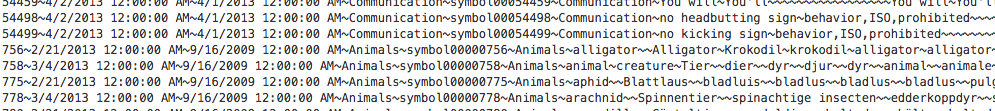
\includegraphics[width=100mm]{datafil} 
\caption{Bilde av dokumentet hvor de ulike symbolene er registrert} 
\label{fig:dok} 
\end{figure} 


\section{Symbol}

Vært objekt i JSON filen og hver linje i tekstfilen blir tolket om til et \textbf{Symbol} objekt. I kontekst av MVVM vil Symbol være en \textit{Model}. Et symbol sine viktigste egenskaper er ordet, stien til bilde som representerer ordet og hvilken kategori ordet tilhører. Den har også egenskaper som synonymer, id, forskjellige språk. Figur \ref{fig:symb} er utdrag fra symboltabellen og viser hvordan 4 symboler ser ut i brukergrensesnittet. De to øverste er ord, mens de to på nederste rad representerer kategorier. Symboler som representerer ord vil alltid ha en hvit bakgrunnsfarge med kategorien den tilhører som kant. Kategorier vil alltid ha en annen enn hvit bakgrunnsfarge. Dette er for at det skal være lettere å skille mellom dem.

 \begin{figure}[ht!] 
\centering 
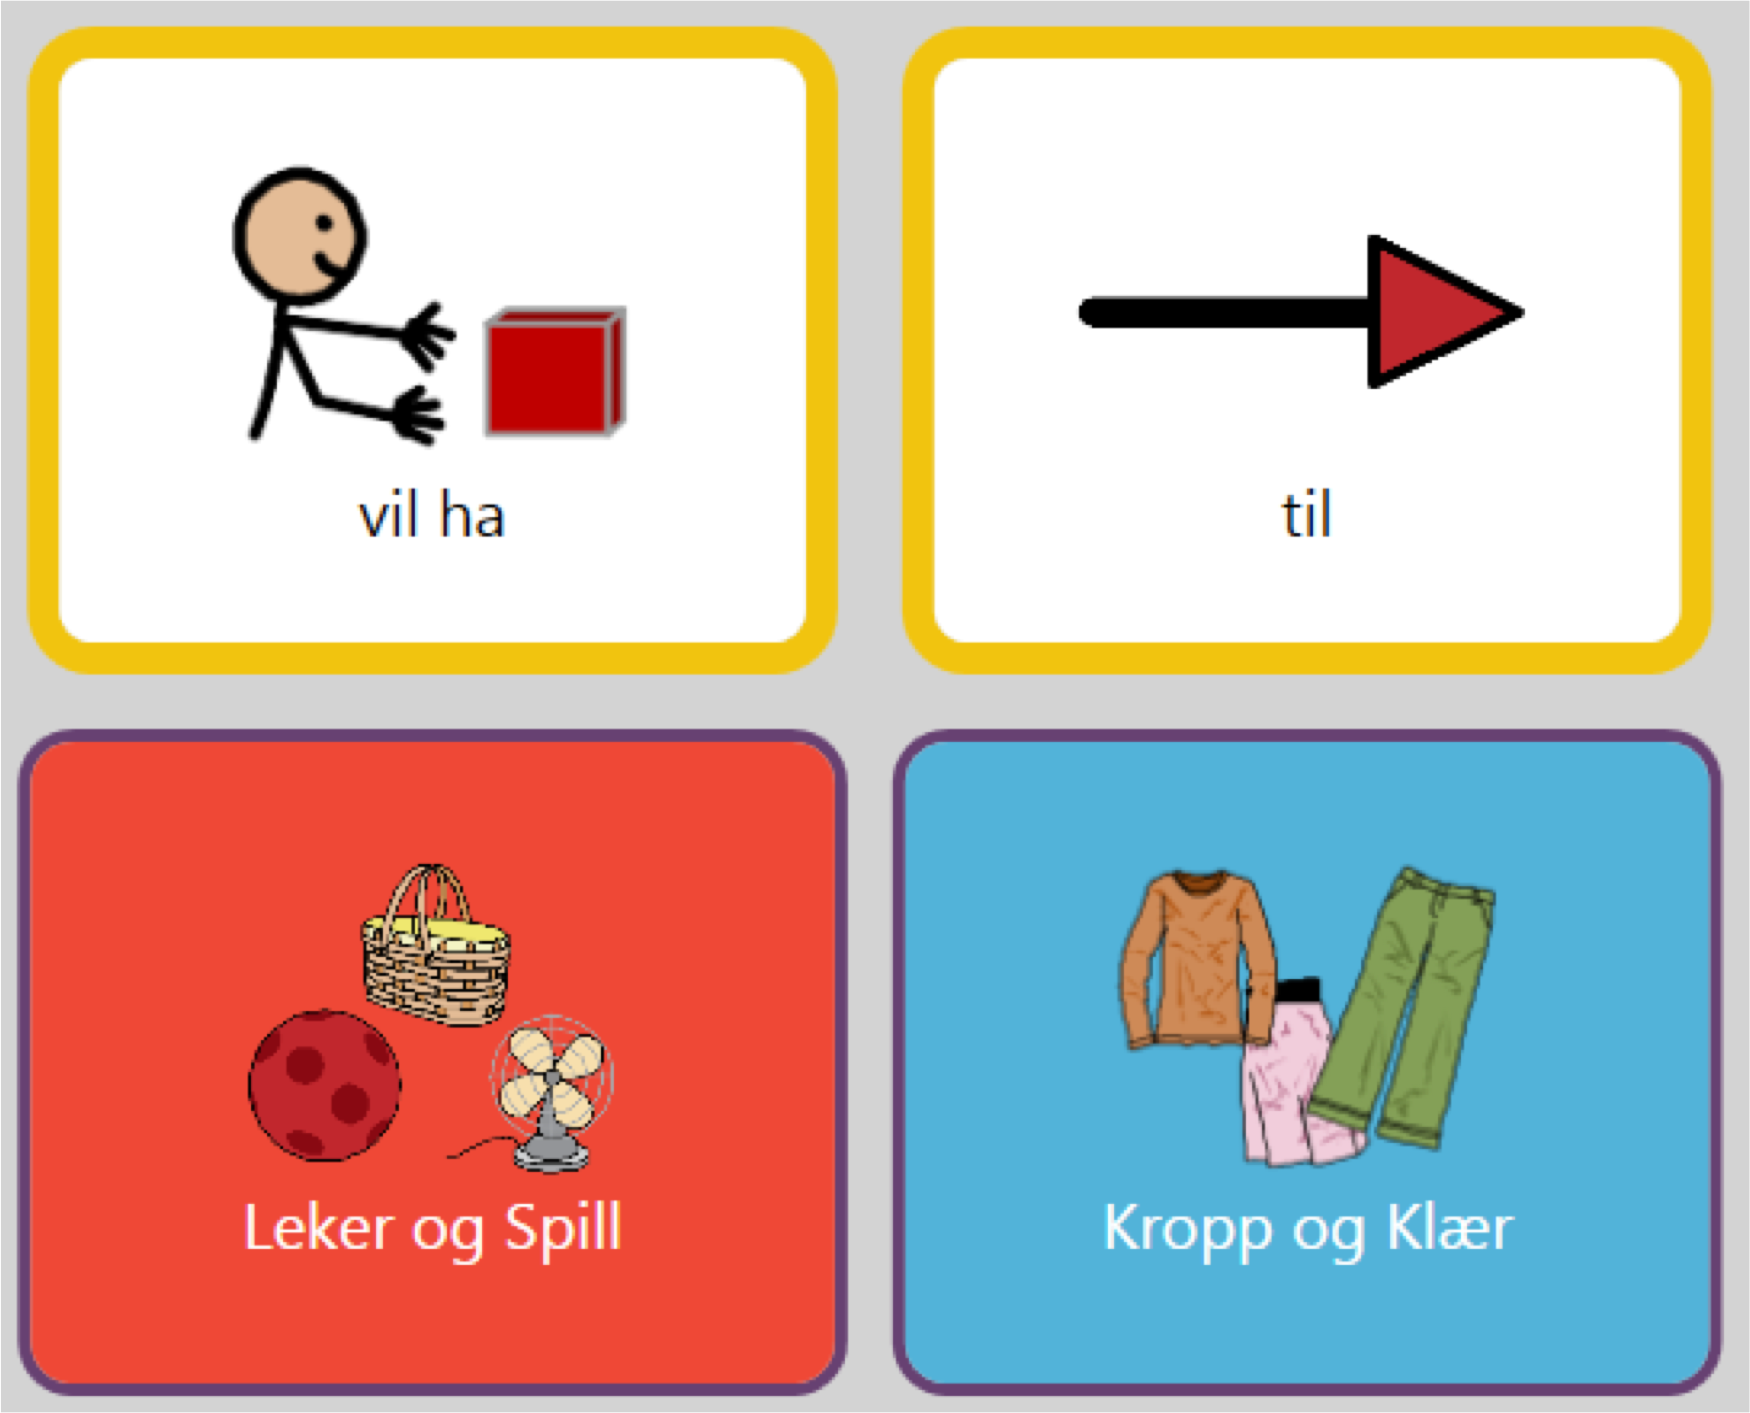
\includegraphics[width=100mm]{Symboler} 
\caption{Fire Symboler vist i brukergrensesnittet} 
\label{fig:symb} 
\end{figure} 

\subsection{SymbolStix}

Bildene som brukes er de samme som i Sono Flex og kommer fra en bildepakke som heter SymbolStix. Dette er en bildepakke som leveres av et eksternt selskap som heter n2y og består av rundt 16 000 symboler \cite{n2y}. Grunnen til at disse bildene ble brukt er fordi det ville tatt for lang tid å lage bilder selv eller å finne dem på nettet, som heller ikke er helt lovlig. Disse bildene har fordelen av at de er laget av profesjonelle noe som ses gjennom den gjennomførte stilen og presise tegninger.


\section{Kategori}

Hver kategori har et navn og en liste over alle symbolene som tilhører den. Eksempelvis så vil symbolene med ord som "hest", "ku" og "hund" ligge i listen til kategorien med navnet "dyr". Figur \ref{fig:katego} viser resultatet ved å trykke på kategorien "dyr". 

\begin{figure}[ht!] 
\centering 
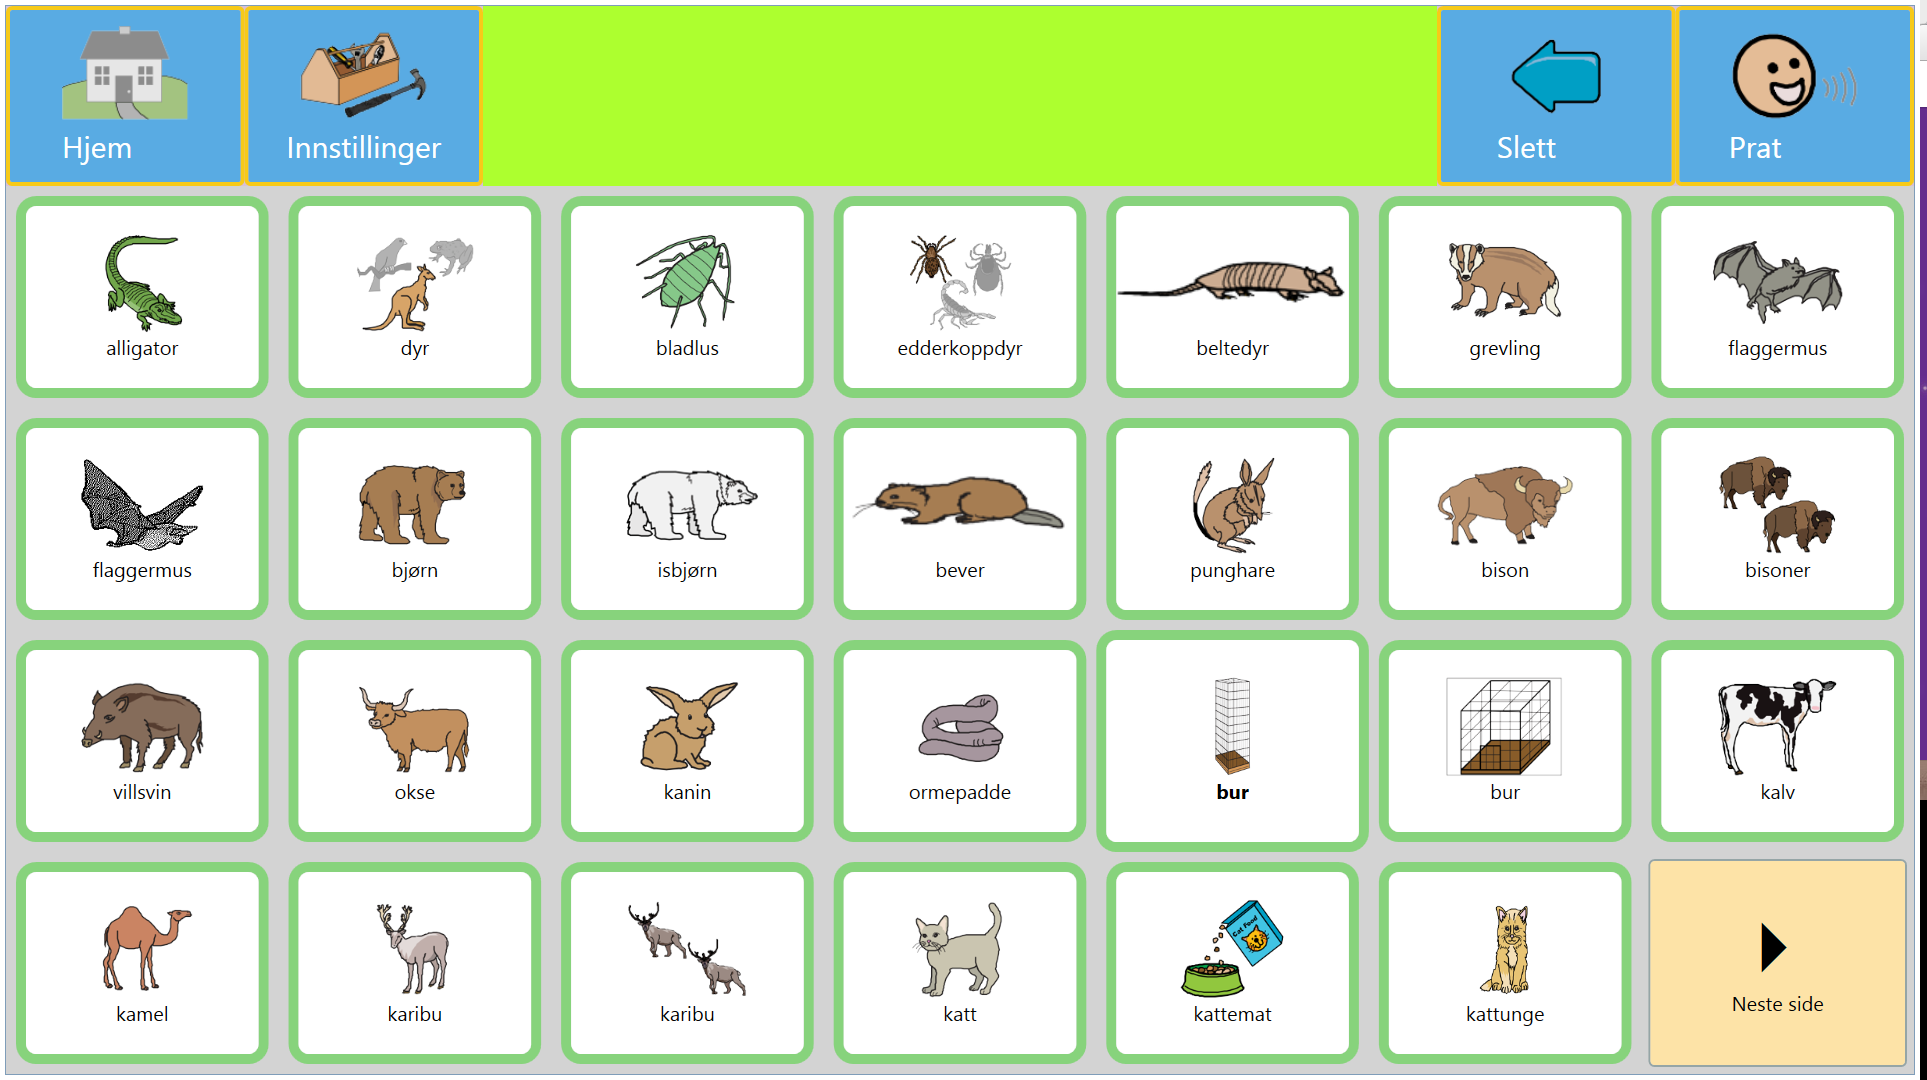
\includegraphics[width=100mm]{dyr} 
\caption{Symbolene på skrivebordet} 
\label{fig:katego} 
\end{figure} 



 
\section{Beskrivelse av prototypen} 

Prototypen har som en kan se fra figur \ref{fig:protooo} den samme layouten som Tobii Sono Flex, med en menylinje etterfulgt av en symboltabell under. Det er derimot en del variasjoner i hver av disse komponentene.  

\begin{figure}[ht!] 
\centering 
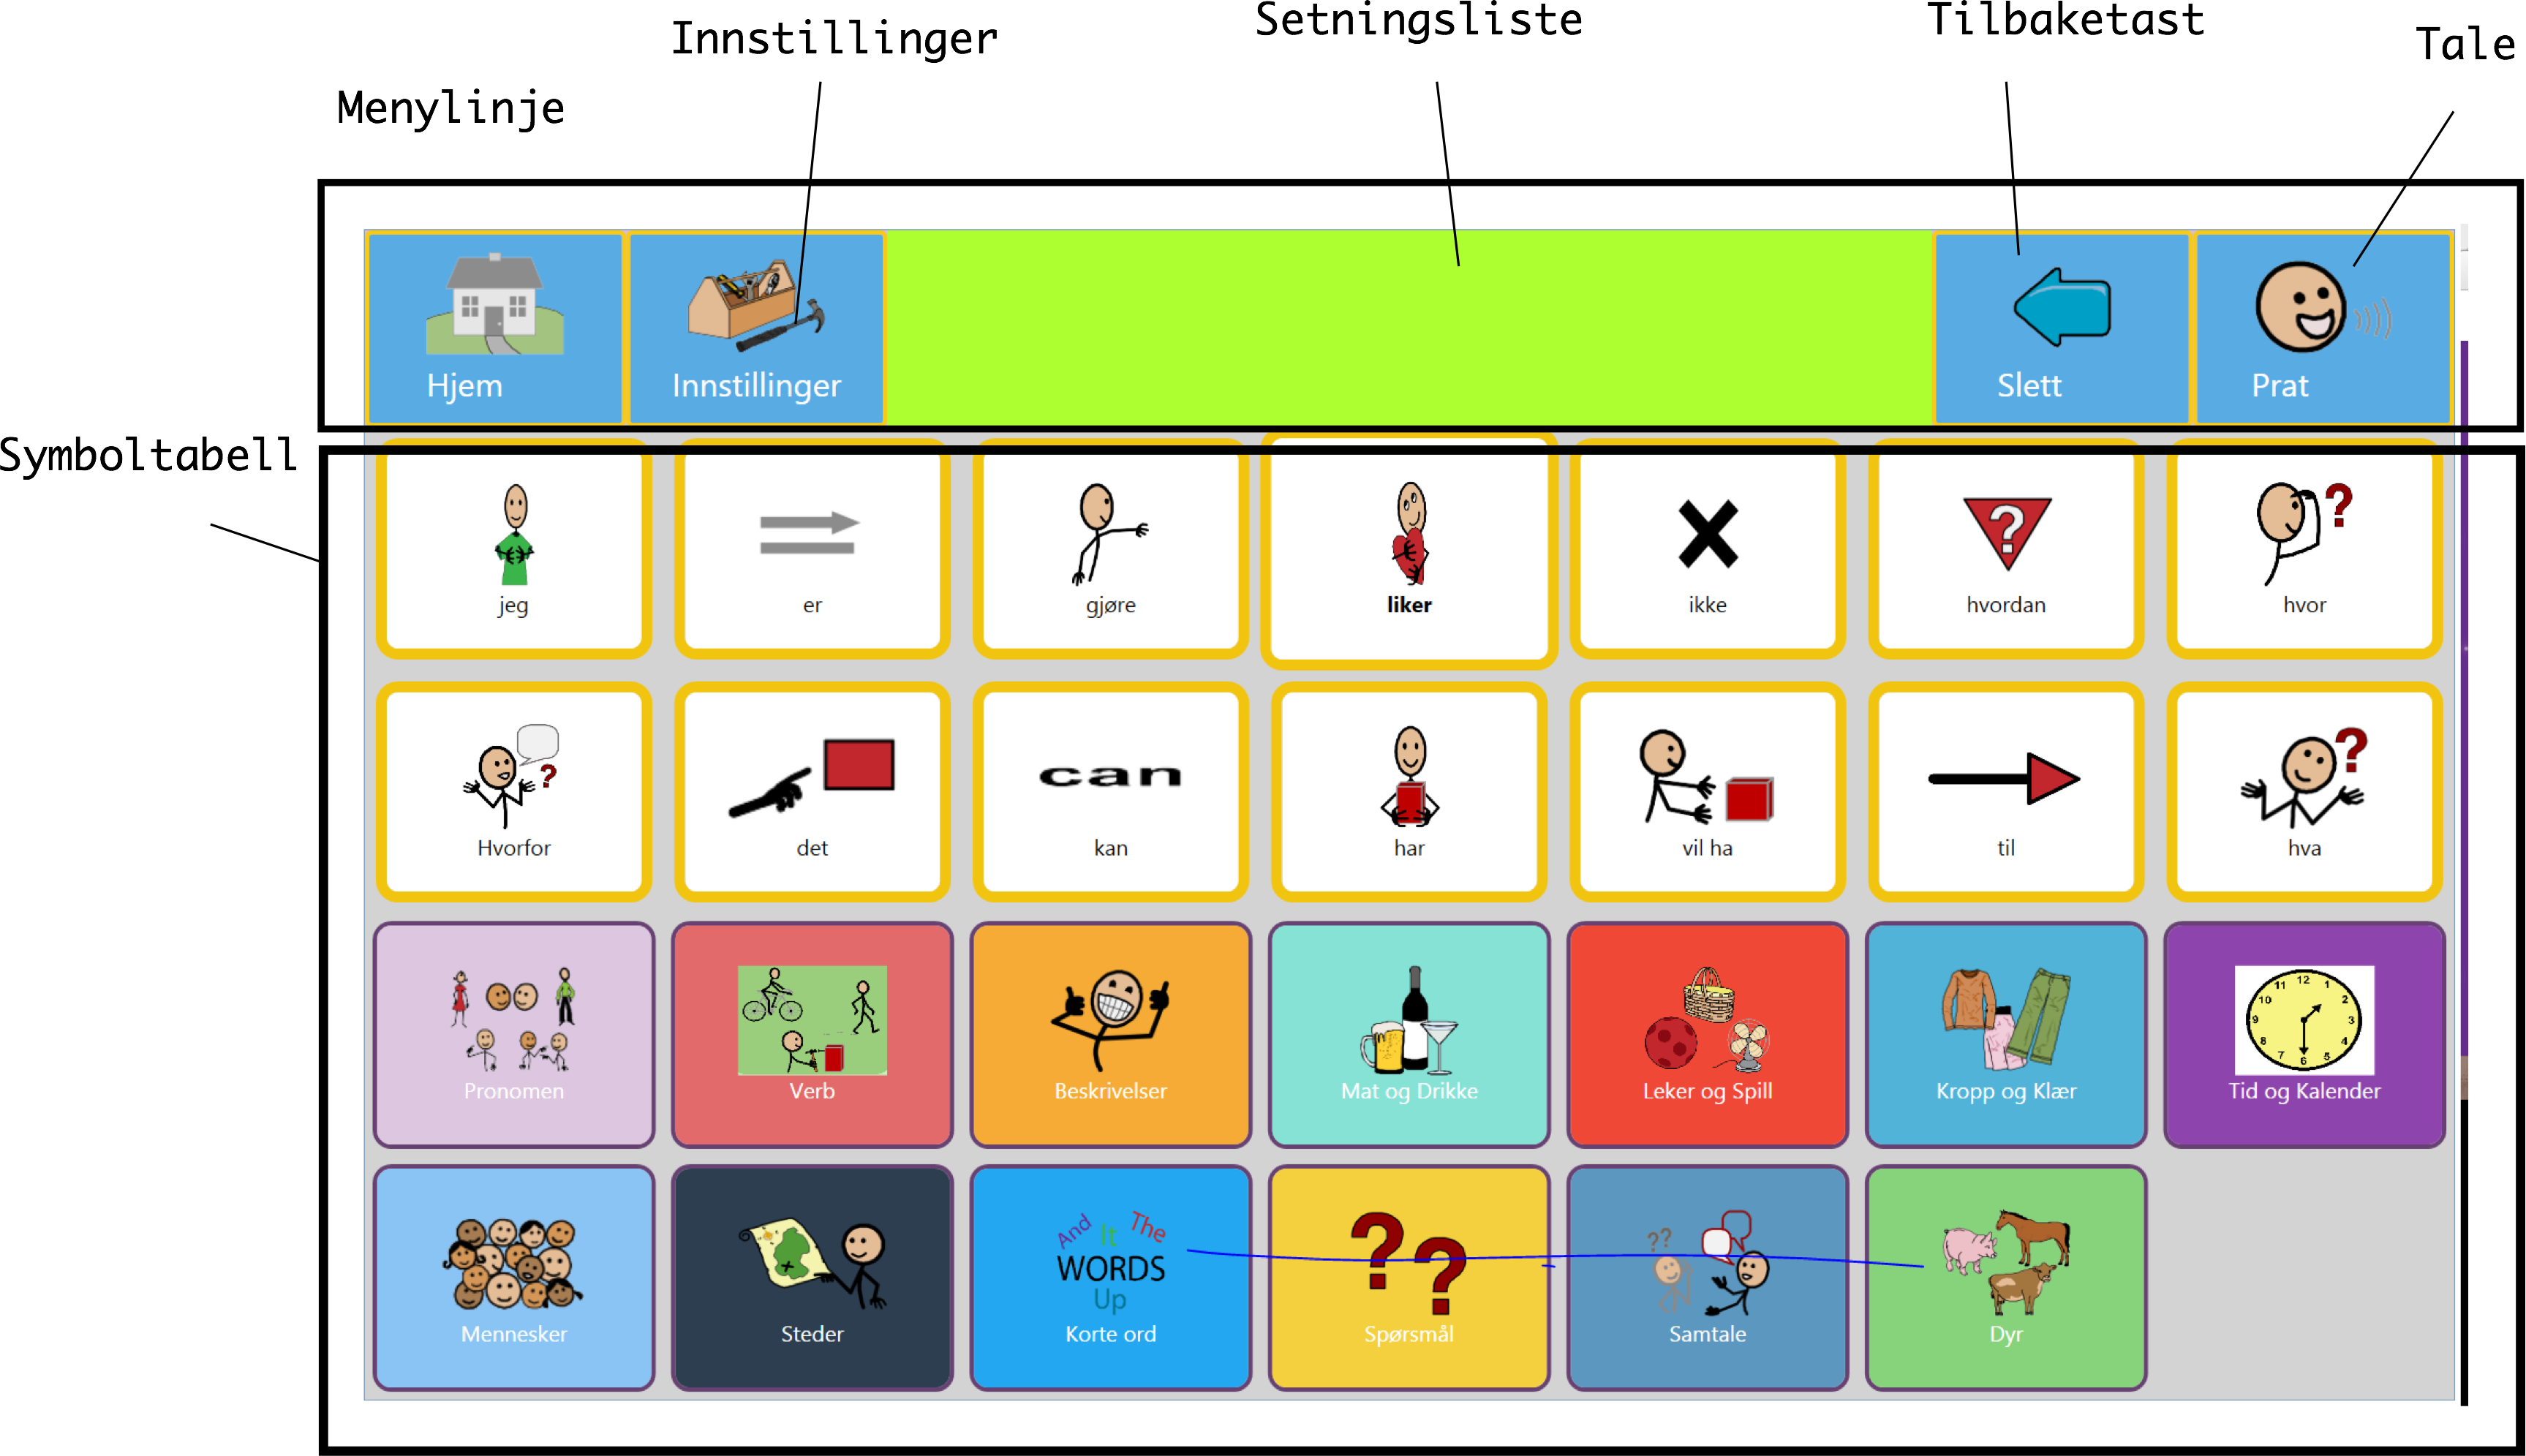
\includegraphics[width=100mm]{ForskjelligeElementerIproto} 
\caption{Prototypen med navn på de ulike delene} 
\label{fig:protooo} 
\end{figure} 


\subsection{Menylinjen} 
 
Menylinjen dekker 1/5 del av applikasjonens vindu og består av 4 knapper og listen over ord som brukeren har trykket på. 
 
\subsubsection{Tilbaketasten} 
 
Tasten som befinner seg til høyre for ordlisten er tilbake tasten. Som på et vanlig tastatur vil et trykk på denne knappen medføre at det siste ordet i ordlisten fjernes. 
 
\subsubsection{Ordlisten} 
 
Når en bruker trykker på et ordsymbol så vil dette legge seg i ordlisten og når han trykker på "prate" knappen så vil ordene i listen bli gitt gjennom høyttalerne som naturlig tale og deretter fjernes fra listen. Selv om det er plass til uendelig med ord i listen så vil det kun være mulig for brukeren å se maks 4 om gangen. Hvis det allerede er fire symboler i listen når brukeren trykker på et nytt symbol, så vil de tre første bli "fjernet" mens det fjerde og det nye symbolet vil være igjen. Hvis brukeren igjen fjerner de to siste ordene ved å trykke på tilbake tasten,  vil ordene som kommer før igjen bli presentert for brukeren i setningslisten.  
 
 
\subsubsection{Hjem} 
Ved å trykke på "hjem" knappen vil brukeren alltid bli ført til førstesiden av applikasjonen uavhengig av hvor han befinner seg.  
 
\subsubsection{Innstillinger} 
Hvis brukeren første er på "hjem" siden av applikasjonen så vil knappen byttes ut med en "innstillinger" knapp. Ved å trykke på denne vil det åpnes et nytt vindu hvor brukeren vil ha mulighet til å sette og endre på diverse innstillinger. Detaljene rundt denne siden er beskrevet i seksjon. 
 
 
\begin{figure}[ht!] 
\centering 
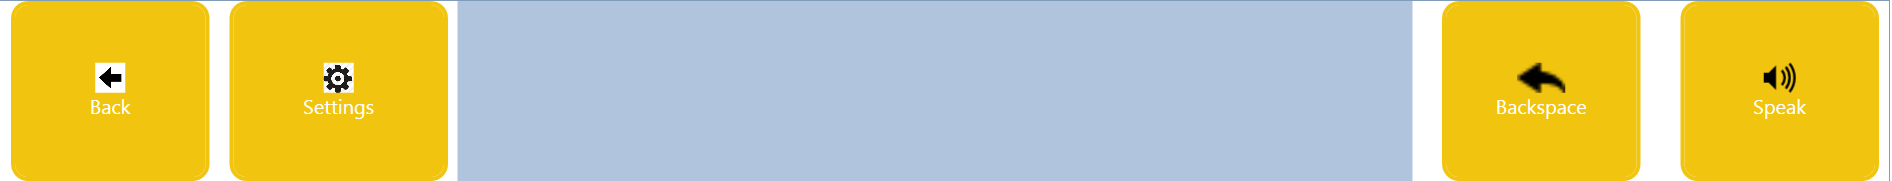
\includegraphics[width=100mm]{MenylinjeP} 
\caption{Skjermdump av menylinjen i prototypen} 
\label{fig:menylinjen} 
\end{figure} 
 



\section{Sammendrag} 

Vi har utviklet en high-fidelity prototype hvor alle kravene i kravspesifikasjonen er oppfylt, noen med mer suksess enn andre. Prototypen er bygget på en moderne plattform som forstatt blir videreutviklet og som har et stort antall tilhengere. Koden skal ved hjelp av flere tiltak være godt tilrettelagt for videreutvikling. 




